\section{Results}
\label{sec:results}

\subsection{Headline accuracy}

\Tabref{tab:main} reports per-cell exact-match accuracy with 95\%
bootstrap confidence intervals for the full $2 \times 2 \times 5$
design. The pattern is clean: \COT lifts both models to 99--100\%
accuracy from $K{=}0$, while \Direct prompting plateaus at 79--93\%
even after eight same-grid demonstrations.
\Figref{fig:rep_curves} plots the same numbers as a function of $K$.

\begin{table}[t]
\centering
\caption{Per-cell exact-match accuracy on \addrtask
($n{=}80$ per cell, 95\% bootstrap CIs). \COT is at or near ceiling
across both models and every $K$; \Direct plateaus well below ceiling.
Best per row in \textbf{bold}.}
\label{tab:main}
\resizebox{\textwidth}{!}{%
\begin{tabular}{@{}llccccc@{}}
\toprule
\textbf{Model} & \textbf{Reasoning} & \textbf{$K{=}0$} & \textbf{$K{=}1$} & \textbf{$K{=}2$} & \textbf{$K{=}4$} & \textbf{$K{=}8$} \\
\midrule
\gpt   & \Direct & 0.788\, {\scriptsize [0.70, 0.88]} & 0.812\, {\scriptsize [0.71, 0.90]} & 0.825\, {\scriptsize [0.74, 0.90]} & 0.850\, {\scriptsize [0.76, 0.93]} & 0.875\, {\scriptsize [0.80, 0.94]} \\
\gpt   & \COT    & \textbf{1.000}\, {\scriptsize [1.00, 1.00]} & 0.988\, {\scriptsize [0.96, 1.00]} & 0.988\, {\scriptsize [0.96, 1.00]} & \textbf{1.000}\, {\scriptsize [1.00, 1.00]} & \textbf{1.000}\, {\scriptsize [1.00, 1.00]} \\
\midrule
\haiku & \Direct & 0.650\, {\scriptsize [0.55, 0.76]} & 0.700\, {\scriptsize [0.60, 0.80]} & 0.762\, {\scriptsize [0.68, 0.85]} & 0.875\, {\scriptsize [0.80, 0.94]} & 0.925\, {\scriptsize [0.88, 0.98]} \\
\haiku & \COT    & \textbf{0.938}\, {\scriptsize [0.88, 0.99]} & \textbf{1.000}\, {\scriptsize [1.00, 1.00]} & \textbf{1.000}\, {\scriptsize [1.00, 1.00]} & \textbf{1.000}\, {\scriptsize [1.00, 1.00]} & \textbf{1.000}\, {\scriptsize [1.00, 1.00]} \\
\bottomrule
\end{tabular}
}
\end{table}

\begin{figure}[t]
\centering
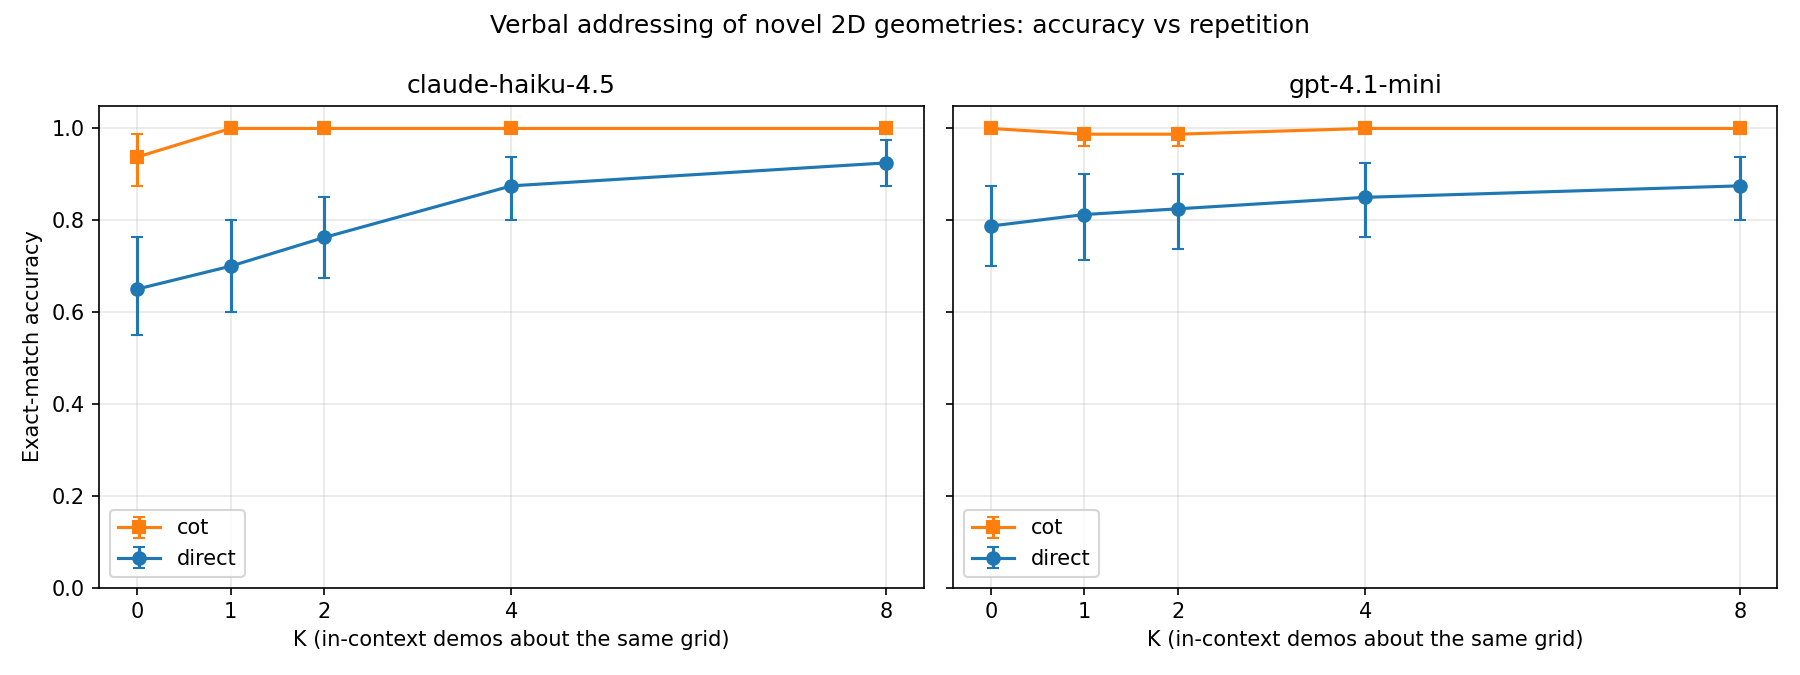
\includegraphics[width=0.85\linewidth]{figures/repetition_curves.png}
\caption{Accuracy on \addrtask as a function of in-context repetition
$K$, for two models $\times$ two prompting regimes. Shaded bands are
95\% bootstrap CIs ($n{=}80$). \COT is at or near ceiling across all
$K$ for both models; \Direct prompting rises with $K$ but plateaus well
below ceiling.}
\label{fig:rep_curves}
\end{figure}

\subsection{Paired \Direct vs.\ \COT tests}

\Tabref{tab:mcnemar} reports McNemar exact tests on the paired
within-item binary outcomes at every $(\text{model}, K)$ cell. \COT
beats \Direct at every one of the ten cells; nine of ten survive the
Bonferroni-corrected threshold $\alpha_i{=}0.005$. The \COT-only
discordant column is uniformly larger than the \Direct-only column at
every cell.

\begin{table}[t]
\centering
\caption{\Direct vs.\ \COT paired McNemar exact tests at every
$(\text{model}, K)$ cell ($n{=}80$ per cell). Discordant pairs are
(\Direct-only correct, \COT-only correct). $\star$ marks rows
significant after Bonferroni correction across the ten tests
($\alpha_{\mathrm{family}}{=}0.05$, $\alpha_i{=}0.005$).}
\label{tab:mcnemar}
\begin{tabular}{@{}llcccrc@{}}
\toprule
\textbf{Model} & \textbf{$K$} & \Direct \textbf{acc} & \COT \textbf{acc} & \textbf{Discordant} & \textbf{McNemar $p$} & \\
\midrule
\gpt   & 0 & 0.788 & 1.000 & (0, 17) & $1.5 \times 10^{-5}$ & $\star$ \\
\gpt   & 1 & 0.812 & 0.988 & (1, 15) & $5.2 \times 10^{-4}$ & $\star$ \\
\gpt   & 2 & 0.825 & 0.988 & (0, 13) & $2.4 \times 10^{-4}$ & $\star$ \\
\gpt   & 4 & 0.850 & 1.000 & (0, 12) & $4.9 \times 10^{-4}$ & $\star$ \\
\gpt   & 8 & 0.875 & 1.000 & (0, 10) & $2.0 \times 10^{-3}$ & $\star$ \\
\midrule
\haiku & 0 & 0.650 & 0.938 & (2, 25) & $5.6 \times 10^{-6}$ & $\star$ \\
\haiku & 1 & 0.700 & 1.000 & (0, 24) & $1.2 \times 10^{-7}$ & $\star$ \\
\haiku & 2 & 0.763 & 1.000 & (0, 19) & $3.8 \times 10^{-6}$ & $\star$ \\
\haiku & 4 & 0.875 & 1.000 & (0, 10) & $2.0 \times 10^{-3}$ & $\star$ \\
\haiku & 8 & 0.925 & 1.000 & (0,  6) & $3.1 \times 10^{-2}$ & \\
\bottomrule
\end{tabular}
\end{table}

\subsection{Effect of repetition}

\Tabref{tab:rep} contrasts $K{=}0$ and $K{=}8$ within each reasoning
condition. For \Direct prompting, repetition matters substantially
(especially for \haiku, $0.650 \to 0.925$, $p<10^{-6}$); for \COT,
both models are already at or near ceiling at $K{=}0$ and there is no
detectable trend. Spearman $\rho$ on $K$ vs.\ correctness confirms
this: \haiku \Direct shows $\rho{=}0.249$ ($p{=}4.8 \times 10^{-7}$),
while \COT trends are weaker and uniformly toward the ceiling.

\begin{table}[t]
\centering
\caption{$K{=}0$ vs.\ $K{=}8$ within reasoning condition (paired
McNemar). $\star$ marks Bonferroni-significant rows
($\alpha_{\mathrm{family}}{=}0.05$, four tests, $\alpha_i{=}0.0125$).
Repetition helps \Direct prompting; \COT is at ceiling so adding demos
has no effect.}
\label{tab:rep}
\begin{tabular}{@{}llccrr@{}}
\toprule
\textbf{Model} & \textbf{Reasoning} & \textbf{Acc $K{=}0$} & \textbf{Acc $K{=}8$} & \textbf{Discordant} & \textbf{McNemar $p$} \\
\midrule
\gpt   & \Direct & 0.788 & 0.875 & (1, 8)   & $3.9 \times 10^{-2}$ \\
\gpt   & \COT    & 1.000 & 1.000 & (0, 0)   & $1.000$ \\
\haiku & \Direct & 0.650 & 0.925 & (0, 22)  & $4.8 \times 10^{-7}\,\star$ \\
\haiku & \COT    & 0.938 & 1.000 & (0, 5)   & $6.3 \times 10^{-2}$ \\
\bottomrule
\end{tabular}
\end{table}

\subsection{Where does \Direct fail? Per-question-type breakdown}

\Tabref{tab:qtype} pools across $K$ and reports the error rate for each
question type, and \Figref{fig:qtype} plots the same numbers as a
heatmap. The pattern is unmistakable: \Direct prompting handles
random-access queries (\qpoint, \qlookup, \qneighbor) at near-ceiling
accuracy, and falls off a cliff on the two aggregation queries
(\qcount, \qrowmax). For \gpt, the \Direct \qcount error rate is
0.675---54 errors out of 80 trials---and on inspection 50 of those 54
are off-by-one---the model registers that the token is present
but loses track of how many. For \haiku, \Direct \qrowmax
errors reach 0.537. \COT eliminates virtually all of these errors.

\begin{table}[t]
\centering
\caption{Error rate by query type, pooled across $K$. Random-access
queries (\qpoint, \qlookup, \qneighbor) are at near-ceiling for both
models under \Direct prompting; aggregation queries (\qcount, \qrowmax)
account for almost the entire \Direct--\COT gap. Bold marks failure
modes (error rate $> 0.1$).}
\label{tab:qtype}
\begin{tabular}{@{}lcccc@{}}
\toprule
\textbf{Query} & \gpt \Direct & \gpt \COT & \haiku \Direct & \haiku \COT \\
\midrule
\qpoint    & 0.000 & 0.000 & 0.075 & 0.013 \\
\qlookup   & 0.000 & 0.013 & 0.087 & 0.000 \\
\qneighbor & 0.050 & 0.000 & 0.025 & 0.000 \\
\qcount    & \textbf{0.675} & 0.013 & \textbf{0.362} & 0.000 \\
\qrowmax   & \textbf{0.125} & 0.000 & \textbf{0.537} & 0.050 \\
\bottomrule
\end{tabular}
\end{table}

\begin{figure}[t]
\centering
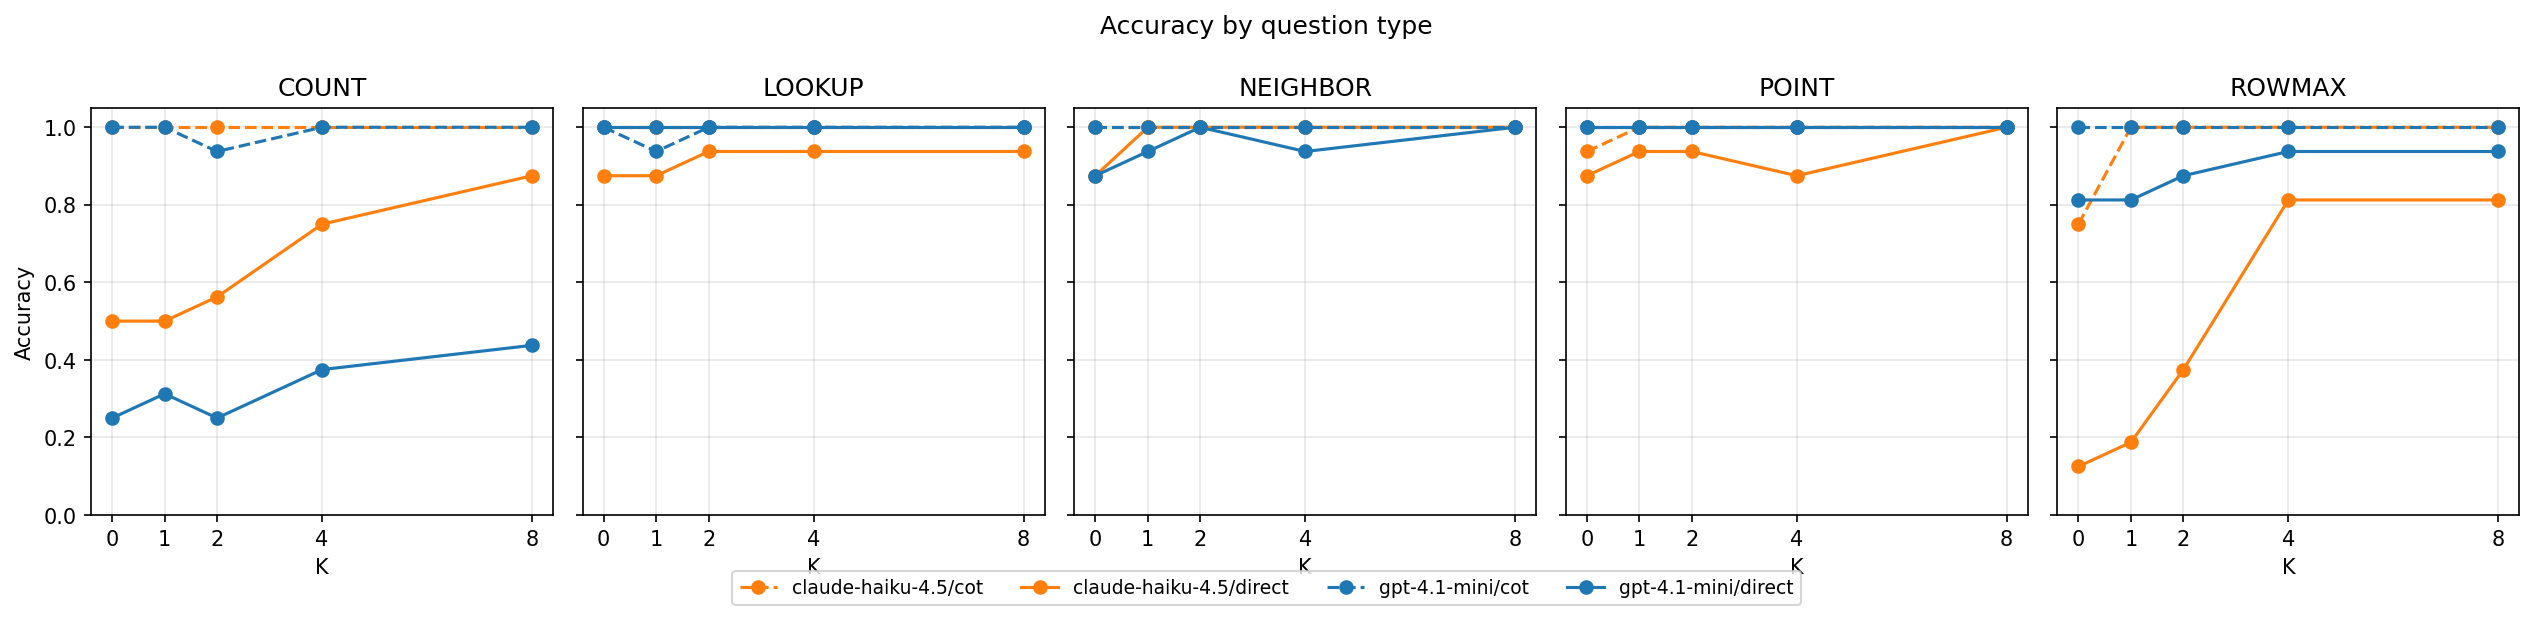
\includegraphics[width=0.9\linewidth]{figures/qtype_breakdown.png}
\caption{Per-query-type error rate for each model $\times$ reasoning
condition, pooled across $K$. Aggregation queries (\qcount, \qrowmax)
account for almost the entire \Direct--\COT gap; random-access queries
are at near-ceiling under \Direct.}
\label{fig:qtype}
\end{figure}

\subsection{Cost-normalised view}

\COT uses 20--80$\times$ more output tokens than \Direct (\gpt:
2~$\to$~125 tokens/call; \haiku: 8~$\to$~180 tokens/call).
\Figref{fig:cost} plots accuracy against mean output tokens per
response. Even at the most generous tokens-per-call accounting, the
absolute accuracy gap (12--35 percentage points) is too large for
\Direct to be preferable on this task at realistic token prices.

\begin{figure}[t]
\centering
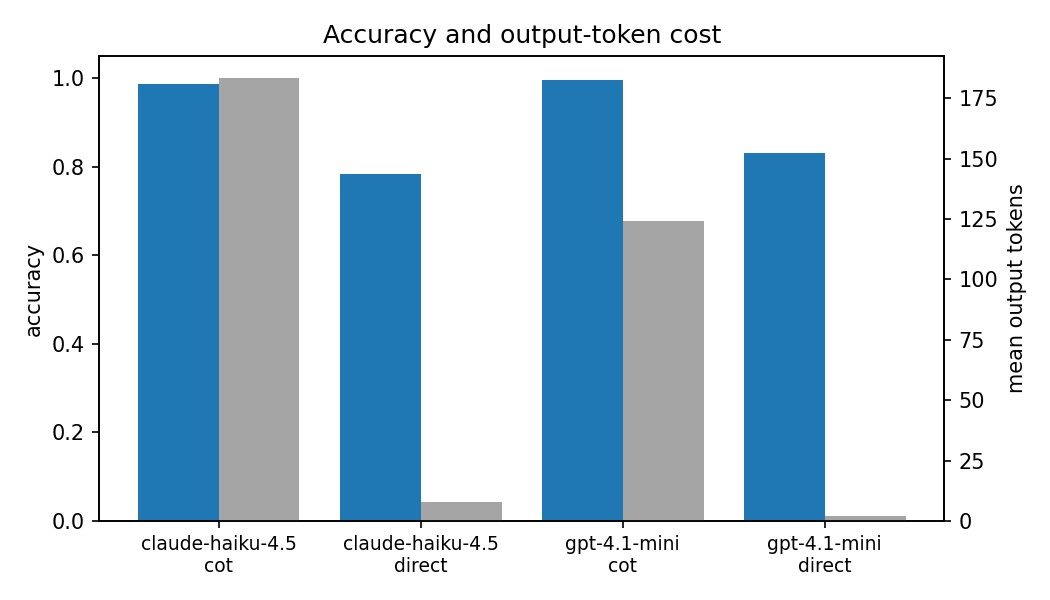
\includegraphics[width=0.75\linewidth]{figures/cost_normalised.png}
\caption{Accuracy on \addrtask vs.\ mean output tokens per response.
\COT uses substantially more tokens but the accuracy gain dominates at
any realistic price ratio. Points show each $(\text{model},
\text{reasoning}, K)$ cell.}
\label{fig:cost}
\end{figure}

\subsection{\miniarc sanity check}

\Tabref{tab:miniarc} reports the rule-induction control. On
\miniarc, \gpt shows the \emph{opposite} ordering from our
addressing task ($\Direct{>}\COT$), consistent with the curse-of-CoT
finding. \haiku exhibits a prompt-compliance failure under \Direct
(it produces reasoning prose that our grid parser cannot extract from
the requested single-grid format), so the \haiku \Direct number is a
floor rather than a capability estimate; we keep the row for
transparency but flag it. The take-away is that our basic setup
reproduces the curse-of-CoT direction in the regime where the
literature predicts it, and the inverted ordering on \addrtask is
therefore not an artefact of the harness.

\begin{table}[t]
\centering
\caption{Secondary \miniarc sanity check ($n{=}25$, no repetition
manipulation). \gpt reproduces curse-of-CoT ($\Direct{>}\COT$); \haiku
\Direct~$=$~0/25 reflects a prompt-compliance failure (the model
emitted reasoning prose our grid parser could not extract), not a
capability finding.}
\label{tab:miniarc}
\begin{tabular}{@{}lcc@{}}
\toprule
\textbf{Model} & \textbf{Direct} & \textbf{CoT} \\
\midrule
\gpt   & \textbf{0.240} & 0.120 \\
\haiku & 0.000$^{\dag}$ & \textbf{0.440} \\
\bottomrule
\end{tabular}
\\[2pt]
{\footnotesize $^{\dag}$Prompt-compliance failure; see text.}
\end{table}
